\section{Arquitectura}
\section{Tecnología}
Para la implementaci\'on de los m\'odulos utilizamos:
	\subsection{Android ADT Bundle} 
		Android ADT Bundle\footnote{ \url{http://developer.android.com/sdk/index.html}} es un paquete provisto por Google que incluye el SDK de Android necesario para compilar las aplicaciones, el entorno de desarrollo Eclipse, con plugins pre-instalados para Android, y un emulador de Android para probar las aplicaciones.
		
	\subsection{Genymotion Android Emulator}
		Genymotion\footnote{\url{http://www.genymotion.com/}} es un emulador de Android que corre sobre Virtual Box usando la arquitectura x86, lo cual permite una performance considerablemente mayor a la del emulador oficial incluido en el Android ADT Bundle, Notamos que podemos correr aplicaciones en Genymotion con la misma velocidad que en un celular real, mientras que con el emulador oficial notamos una performance muy pobre que dificulta el testeo. Usamos también un plugin de Eclipse para Genymotion que nos permite lanzar la aplicación compilada desde la IDE al igual que en el emulador oficial.
		
	\subsection{Sinatra}
		Sinatra\footnote{\url{http://www.sinatrarb.com/}} es un framework de Ruby que permite crear aplicaciones web muy fácilmente y con muy poco código. La usamos porque el servidor que usan nuestras aplicaciones es bastante simple, y sólo recibe y guarda datos de las víctimas. Otras ventajas de Sinatra es que es distribuible, fácil de mantener y extensible.

\section{Arquitectura}
La descomposici\'on de la arquitectura se puede visualizar en el siguiente diagrama:

\begin{minipage}{1.0\textwidth}
    \centering
    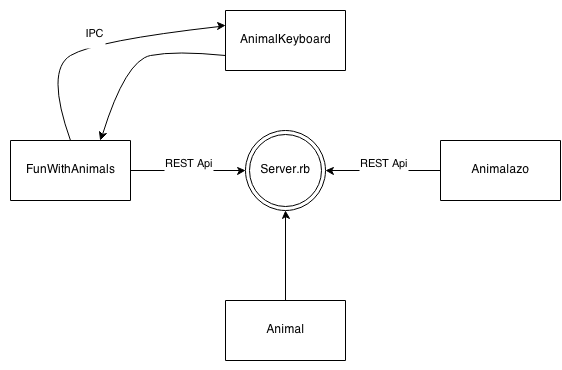
\includegraphics[width=.7\linewidth]{arquitectura}
\end{minipage}%



Donde se visualizan los modulos principales desarrollados y la interacci\'on de estos con el servidor de contenidos.

La API del servidor mediante el cual se interconectan los m\'odulos cuenta con las siguientes operaciones soportadas:


\begin{lstlisting}
get '/contacts' do | res| ...
post '/upload' do ...
post '/key' do ...

\end{lstlisting}

Donde:

\begin{description}
    \item[contacts] que recibe utilizando un GET la lista de contactos y la persiste en un archivo
    \item[upload] que recibe las imagenes y las persiste
    \item [key] que salva los key-strokes presionados por el usuario
\end{description}

